\title{POM}

\documentclass[12pt]{article}

\newcommand{\ra}{$\rightarrow \text{ }$}
\newcommand{\nii}{\noindent}
\usepackage{import}
\usepackage{xifthen}
\usepackage{pdfpages}
\usepackage{transparent}
\usepackage{float}
\usepackage{tcolorbox}
\usepackage{amsmath}
\usepackage{kotex}

\setlength{\parindent}{0em}
\begin{document}

\maketitle

\section{Introduction to Marketing}

What is marketing? Well, one can talk about this in various different way, but let's start with the word itself.
$$ \text{Market}+\text{ing} $$

As the word implies, it can be seen as "doing the market", or, trying to be better with dealing markets. Therefore one can say that marketing is

\begin{tcolorbox}
		\text{Any transaction between Producer and Consumer to Promote trading}
\end{tcolorbox}

That makes marketing to be seen as "Trading Obstacles Elimination Process". What kinds of obstacles are there? More specifically, what can bee seen as obstacle? Obstacle is anything that seperates from Producer and consumer(Under condition that, of course, consumer wants to consume and producer want to produce). It can be relabeled as "Distance obstacle factor". There are 4 main factors.
\begin{itemize}
	\item form
	\item ownership
	\item placement
	\item time
\end{itemize}
The main task of marketing therefore can be seen as eliminating these factors. For this 4 possible following tasks can be stated.
\begin{itemize}
	\item Make product that consumer wants
	\item Make it noticeable by people
	\item Solve the possible causes that make buying difficult.
	\item Keep the continual trading relationship.
\end{itemize}
To actually solve this task, we have \textbf{4P \& STP}. Also we wish to have
an overall management system to sustain these tasks. This is called "Market Research Monitoring"


% \begin{figure}[H]
% 	\centering
% 	\def\svgwidth{\columnwidth}
% 	\import{./figures/}{marketingmanagement.pdf_tex}
% 	\caption{marketingmanagement}
% 	\label{fig:marketingmanagement}
% \end{figure}



C. SWOT analysis

1. Basic Model

BCG Model

The Purpose of BCG matrix: Set the balance of Cash Flow.
\begin{figure}[H]
	\centering
	\def\svgwidth{\columnwidth}
	\import{./figures/}{BCG.pdf_tex}
	\caption{BCG}
	\label{fig:BCG Model}
\end{figure}

Problem of BCG Model

\begin{itemize}
  \item Way too simple x, y cord.
  \item Vague definition of market.
  \item Vague borderline of MGR, H/L
  \item Considers only present state.
  \item Can be too drastic.
  \item Don't consider any synergic possibilities.
\end{itemize}

1) X as "Position of competition" Y as "Attractiveness of Business"

2) Define market within realm of SUB

3) High - Medium - Low

%9월 11일

\section{Marketing research}

\subsection{Topics of Marketing research}

1. Analyzing Situation
\begin{itemize}
	\item Changes in Inside, outside Environments
	\item strength, weakness of our, opponent companies
	\item catching opportunities/analyzing market character
	\item analyzing consumers
\end{itemize}

2. Collecting strategies step
\begin{itemize}
	\item researching consumer's cognition
	\item market test (concept, elasticity of price, predict demand)
	\item
\end{itemize}

3. Strategies acquiring step
\begin{itemize}
	\item add tracking
	\item new product tracking (recognition, preference ... )
\end{itemize}

4. Evaluate step
market share, mind share, brand equity, satisfaction



How do we get the data?
\begin{enumerate}
	\item Search for it (online, researches...)
	\item Make them!
	\item Buy them! (or let other make them)
\end{enumerate}

\subsection{Marketing research process}

\begin{enumerate}
	\item Decide whether we need to research
	\item Specify why we need to research (What are you trying to get by this research?)
	\item type of Constructions of research
	\item Data Source (Do we make them? search for it? etc..)
	\item How do we collect our data?
	\item Extract samples and collect Data (what is our sample group? how? how many?)
	\item Analysis of our data
	\item Result and organize the product.
\end{enumerate}

\subsubsection{Type of research construction}
\begin{enumerate}
	\item Exploratory research
	\begin{itemize}
		\item "Why do we lack net profit?"
		\item "would single family's consuming mind different?"
	\end{itemize}
	\item Descriptive research (much more enumerative and analytical, more to correlational study)
	\begin{itemize}
		\item "Is the reason of lack of net profit differ by different areas?"
		\item "Is the single family consumer sentiment differ by different age?"
	\end{itemize}
	\item Causal research (not much correlational, more causality research)
	\begin{itemize}
		\item "Is price discount better than quantity discount?"
		\item "Is minimalization better than advancing?"
	\end{itemize}
%Class 4_: 오후 3시 50분 ~ 4시 20분 사이 (탐색, 기술, 인과 조사 설명들...)

\end{enumerate}
\subsubsection{Data source}
\begin{enumerate}
	\item Secondary Data
	\begin{itemize}
		\item Inside data (Business related data..)
	\end{itemize}
	\item Primary data
	\begin{itemize}
		\item survey, test
		\item observation, ...
	\end{itemize}
	\item New raw Data
	\begin{itemize}
		\item Purchase Data
		\item clickstream Data
		\item UCC, SNS Data
		\item Big data (3V's)
	\end{itemize}
\end{enumerate}

\subsubsection{Example: Coke or Pepsi?}

Pepsi Challenge

"New coke" blunder

Despite all the research, why did so many people hate New coke?

"are you sure that taste only comes with tongue?"

By doing fMRI study of brain, one can find out that while blind testing, VMPFC of brain was triggered, while drinking coke, DLPFC and Hippocampus was triggered.

\subsubsection{Method of collecting Data}

\begin{enumerate}
	\item collecting Method
	\begin{itemize}
		\item face-to-face/or not
		\item mail, phone
		\item online
		\item mobile
	\end{itemize}
	\item Sampling
	\begin{itemize}
		\item sampling frame
		\item method of sampling (random sampling/easy sampling)
		\item sampling size
	\end{itemize}
\end{enumerate}


\section{Consumer Behavior Analysis}
\subsection{consumer behavior analysis tool}
1. Understanding consumer
\begin{itemize}
	\item who?
	\item what would they want?
	\item How would they react?
	\item why?
\end{itemize}

2. Decision making step
\begin{enumerate}
	\item facing the problem
	\item searching for information
	\item look for alternative
	\item Buying the product
	\item Action after buying product (usage and feedback)

\end{enumerate}

who would face the problem? not exactly the one who uses. can be parent, related people... etc..
Who would search for alternative? Thus, above order can be done by all separate people.
The 2. can be questioned by 1. therefore 20 questions can arise in total. However, the 1. can be much more descriptive.

Personal traits can be influential to Decision steps. This can be,
\begin{itemize}
	\item Memory
	\item attitude.
	\item etc...
\end{itemize}

\subsection{Consumer Behavior's general characteristic}

However, every consumer is human, therefore behaves in very "generalizable" way. It is natural to think that people behave in calculative, rational way. But this turned out to be very wrong.

\begin{enumerate}
	\item Decision making method routinized
	\begin{itemize}
		\item Extensive problem solving (Searching for all possible solution)
		\item Limited problem solving
		\item Routinized behavior
	\end{itemize}
	\item Behaviors within relationships(Between other objective beings)
	\begin{itemize}
		\item Reference group influence (e.g. by pressure, I'm now fine with alcohol)
		\item Trickle down Effect
		There are differences between social hierarchy within behavior of consumers. So called "lower class" tends to follow "higher class"
		\item Social modeling (People tends to follow other people in general. especially who they admire)
		Why is it that, despite not believing the model is only working for "money", the influence is still there. This works for other examples not bounded by human models.
		\begin{figure}[H]
	\centering
	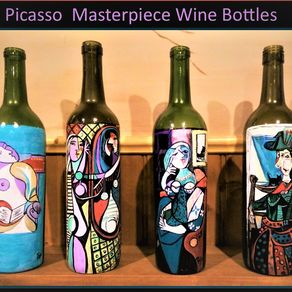
\includegraphics[width=0.95\textwidth]{img/picawine.png}
	\caption{Wine bottle with image of Picasso sells dramatically}
	\label{}
\end{figure}

	\end{itemize}
	\item Expected Irrationality (We are very irrational indeed, but we are irrational in very rational way. Therefore, pre-calculatable)
	\begin{itemize}
		\item Heuristics and biases
		\item  Emotional decisions
		\item Non conscious behaviors (Done without conscious)
	\end{itemize}
\end{enumerate}
Theses behaviors can be (in a way) predicted by marketers, making marketing process much efficient.
How many of us make un-rational decisions? about 80\%, says our professor.

\begin{figure}[H]
	\centering
	\def\svgwidth{\columnwidth}
	\import{./figures/}{consumerMotivation.pdf_tex}
	\caption{What drives consumer Motivation?}
	\label{fig:consumerMotivation}
\end{figure}

\subsubsection{Consumer Behavior's Megatrend (keyword)}
\begin{itemize}
	\item Consumer rights
	\item Produmer (producer and both consumer)
	\item Life's quality (well being, health, prestige, small luxury)
	\item Green Friendly (ethical, green, shared consumption)
	\item High-Tech (Mobile, AI, IoT, VR, Robot)
	\item Decision disorder (info overload, decision curator)
\end{itemize}

\section{Segmentation and Targeting}

How do we actually "Do" marketing?

\subsection{Segmentation}

definition: splitting the market into few 'segments'
But do we really need market segmentation?

\subsubsection{Necessity of Market Segmentation}

First, the customers are very different. \ra You can be very precise to customer's needs
Also, the company has very limited resources. \ra You can choose and focus on one point.
And finally, there are just too much competition.
Segmenting makes different opportunities stand out
very easily.
Plus, you can also act very quickly to changes.

\begin{figure}[H]
	\centering
	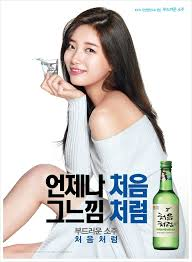
\includegraphics[width=0.95\textwidth]{img/soju.png}
	\caption{Target market : Easily enjoying liquor, for age 20 ~ 30, woman, lives in cities.}
	\label{soju}
\end{figure}


\subsubsection{Standards for Market segmentation}

\begin{itemize}
	\item Geological variable \ra weather, pop density, areas
	\item Demographic variable \ra age, gender, income level, educational, job
	\item Physiological variable \ra Values, personality traits, motivation, lifestyle
	\item Behavioral variable \ra Pursuit of convenience , amount of usage, preferences, bargaining
\end{itemize}

\textbf{Geological, Populational-statistical Variable \\ (Demographic variable)}

\begin{itemize}
	\item Sometimes define the demand for entire category!! (weather, population, age, gender, income level)
	\item Creates \textbf{subculture} (Generation wise, jobwise, area wise culture)
	\item Customer Porfile elements \ra "accessibility" (who are they? How do we(company) approach them?)
\end{itemize}

\begin{tcolorbox}
	\textbf{Example}: Cookies (HaeTae and Lotte)
	\begin{center}
		Do cookies really need market segmentation?
	\end{center}
	You can make an argument that everyone likes cookies. Almost everyone consumes cookies. Yet, there seemed to be \textbf{geological difference} between areas. Why is that? Even though heavy consumers are children, it seemed like area's conflict seemed to be engaged: Therefore focus on the \textbf{distributor}. Thing are getting better nowdays. link:
	http://www.donga.com/news/article/all/20030826/7976875/1

\end{tcolorbox}

\textbf{Physiological Variable:}
\begin{itemize}
	\item Effects almost every aspect of consumer's behavior (values, personality traits, lifestyle etc...)
	\item One of the Customer's profile's elements : \ra Appealing methods (How do we invoke consumer's motivation to buy?)
\end{itemize}
\textbf{Question: How do you segment market by personal values?}

\subsubsection{LOV Segmentation}

1. Main Value measurement
\begin{itemize}
	\item  Rokeach survay (36 value items)
	\item List of value (LOV) (9 value items)

\end{itemize}
\nii
2. Rounding off by main values \ra \textbf{Factor analysis}
\nii
3.Making Segments \ra \textbf{Clustering analysis}

\begin{tcolorbox}
	How do you exactly make factor analysis?
	% 자긍, 자아실현, 성취 존경 : factor 1
	% 존겨으 재미, 흥 : factor 2
	% 안저으 소속, 대인관계: factor 3
\end{tcolorbox}

After factor analysis, you make clustering by looking at the data.

% \begin{figure}[H]
% 	\centering
% 	\def\svgwidth{\columnwidth}
% 	\import{./figures/}{clustering.pdf_tex}
% 	\caption{Clustering}
% 	\label{fig:clustering}
% \end{figure}

Behavioral Variable

\begin{itemize}
	\item Craving product benefit
	\item Heavy user/ Light user
	\item Reaction Step: (recognition\ra knowledge \ra preferable \ra buying experience \ra recursive purchase)
	if everyone likes it and nobody buys it, there must be purchase obstacle.
	if nobody knows it, must let them know first.
	if everyone know it but nobody likes it, change their attitude.
	etc etc...
	\item price sensitivity
	\item Usage situation: ( Where do people use our product?)
	\item Accepting innovative product (Would they buy beta version?)

\end{itemize}

{\large In what variable do we use to segment market?}

* \textbf{Let's think...}
\begin{enumerate}
	\item Using any standard, market does get segmented. (Now is it just matter of your choice?)
	\item You simply can't use all the standards, because it isn't profitable and way too complicated. \ra \textbf{use right amount}
	\item Thus you need \textbf{Efficient market segmenntation}
\end{enumerate}

\subsection{Effective Market Segmentation}
{\large Effectiveness:::
\begin{enumerate}
	\item Measurable %What??
	\item Accessible
	\item Substantial (Segmented by 99 : 1 is just meaningless.)
	\item Differentiable by segments (if stratagies amoung segemnst are equal, it is meaningless)
\end{enumerate}
}
\ra Yet, \textbf{per variable, Effectiveness is different.} %어떤 변수는 이런 쪽에서 효율이 좋지만 이런 쪽에선 안좋음

\subsubsection{How do you deal with that? Wedel \& Kamakura's}

% \begin{tabular}{c|cc}
% 	\hline
% 	& gneral character variable & Prdouct related variable \\
% 	\hline
%
%
% \end{tabular}
%
% \begin{tabular}{|c|c|c|c|c|}
% 	\hline
% 	 & G/O & G/NO & P/O & P/NO \\
%
% \end{tabular}

{\large Then what??}

\begin{itemize}
	\item Use Multiple Variable
	\item Actionable Variable
	\item use high - Accesiable variable to make profile.
\end{itemize}

\subsection{Steps for Market Segmentation}

\begin{enumerate}
	\item Collect Data
	\item Measure variable by marketing search
	\item %%search later
\end{enumerate}


	Toothpaste Market:

\begin{tcolorbox}
	Product benifit can be very different


\end{tcolorbox}

\subsection{Time variant Segmentation}

How do you segment markets? Well, after fully knowing the method, you still don't know what will come out as an result, nor what is really efficient.
Knowing certain stuff beforehand can be described as \textbf{a priori segmentation}, other is \textbf{a posterirer segmentation}
\begin{figure}[H]
	\centering
	\def\svgwidth{\columnwidth}
	\import{./figures/}{mseapr.pdf_tex}
	\caption{Different segment}
	\label{fig:mseapr}
\end{figure}
For example LOV, you knew how you choose the segmenting method, but you didn't know the result. The result of 4 factor can be considerd as a posterirer.


\section{Targeting}

Ok. you've segmented the market. (that was hard) Now you have to choose what part of segemtn you are going to be engaging in.

\subsection{Target segment's decision standard}

\subsubsection{Segment's attractiveness}
\begin{itemize}
	\item Outside conditions (market size, potential, growth rate, product's life cycle, seasonal)
	\item Structural condition (competition difficulty, threat of alternatives, power of buyer/producer, Wall of entrance(진입장벽))
	\item Environmental condition (Economy, society, ...)
\end{itemize}
\subsubsection{Relative competitive position within the segment}

\begin{itemize}
	\item %차별화 우위
	\item %item
\end{itemize}
{\large The way "competition" is defined can be various}
\nii
\begin{itemize}
	\item By brand (e.g: Digital Camera 1 vs Digital Camera 2)
	\item Form of product {e.g: Digital Camera vs DSLR vs Mirrorless}
	\item Fundamental convenience (e.g: D.c vs Phone)
\end{itemize}
\nii
Ask first brand's most risky competitor

\begin{tcolorbox}
	\begin{itemize}
		\item chmisul \ra samsung TV
		\item Liniage \ra America Drama
		\item sulwhasu \ra Korean medic
		\item Bakcas \ra Starbucks
		\item Nike \ra Nintendo
	\end{itemize}
\end{tcolorbox}

{\Huge \textbf{Marketing Myopia}}
\ra look at market from far direction. ( Would above competition make sense?)
he Fundamental values can be given by much different product.
\subsubsection{Compatibility}
with...
\begin{itemize}
	\item company resources
	\item company's mission/culture
	\item existing market, existing marketing mix.
\end{itemize}

Target market can be
\begin{itemize}
	\item differentiated into one or more segments.
	\item treated as same or different
\end{itemize}

\subsection{Treating differnt: How much?}
\begin{itemize}
	\item
\end{itemize}

\section{Postitioning}
Definition: finding postition inside consumer's \textbf{mind}

\begin{itemize}
	\item competitive differentiation consumer perceive
	\item problem of competitive structure's overall harmonizing marketing mix.
	\item Not reality, just perception
	\item Can define direct competitors
	\item Can grasp market oppurtunities
\end{itemize}
\subsection{Positioning Map}

\begin{figure}[H]
	\centering
	\def\svgwidth{\columnwidth}
	\import{./figures/}{pmap.pdf_tex}
	\caption{Structure of positioning map}
	\label{fig:pmap}
\end{figure}
\subsubsection{Making of positioning map}
\begin{enumerate}
	\item Multi Attribute Model (MAM)
	\ra what constitutes a product is used as axis. (and how good they are per product of different companies)
	\item Multi Dimensional Scaling (MDS)
	\ra Asking consumers for unknown axis, and trying to search for axis.
\end{enumerate}

1. MAM
\begin{itemize}
	\item grasp main character of products.
	\item Per product, find the values for characters.
	\item Factor Analysis
	\begin{itemize}
		\item figuring out the underlying dimensions
		\item find the scale value per theses basis dimension.
	\end{itemize}
	\item  Make positioning map.
\end{itemize}

2. MDS
\begin{tcolorbox}
	"Making positioning map under recognition of consumer's similarity"

\end{tcolorbox}
Ask customer's their measure of similarity of different products.

\begin{figure}[H]
	\centering
	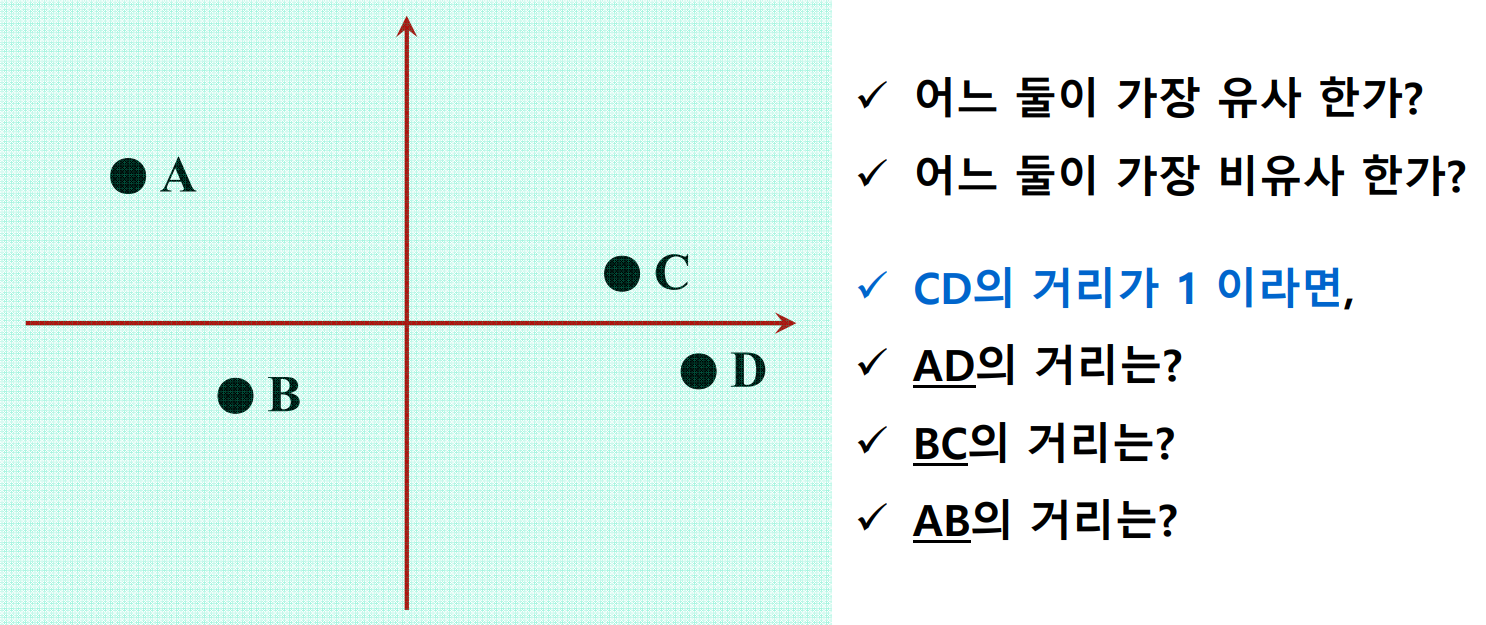
\includegraphics[width=0.95\textwidth]{img/mds.png}
	\caption{}
	\label{}
\end{figure}

\subsection{Positioning Strategy}
\begin{enumerate}
	\item Overall Quality - Price positioning
	\item Specific POD(point of difference) positioning
	\item condition of Efficient positioning
\end{enumerate}
\subsection{Overall Quality - Price positioning}
\begin{figure}[H]
	\centering
	\def\svgwidth{\columnwidth}
	\import{./figures/}{oqpp.pdf_tex}
	\caption{}
	\label{fig:oqpp}
\end{figure}
\subsection{Specific POD(point of difference) positioning}
\begin{itemize}
	\item property POD
	\item Service POD
	\item User POD
	\item Usage situation POD
\end{itemize}
{\large Many time, positioning is done with specific property POD}

But sometimes, user specific POD is done. (풀무원:(환경친화적인 당신은) 이미 풀무원입니다)

\subsection{Efficient POD condition}
\begin{enumerate}
	\item POD's dimension is important
	\item That difference must be perceived meaningfully
\end{enumerate}

\begin{center}
	Meaningful POD vs not! meaningful POD

\end{center}
\begin{enumerate}
	\item Work in existing field,\ra make strategies within known map
	\begin{itemize}
		\item difference within already existing dimension
		\item comparing quality between other competitors ("alignable" difference)
		\item Property - based POD is almost all this case
	\end{itemize}
	\item Change the existing field \ra taking strategies to change the existing map
\end{enumerate}
\subsubsection{make strategies within known map}
Here, the specific dimension is very important, but the problem is that "challenger's" claim isn't well informed.
\begin{itemize}
	\item Most of the difference is ignored (Prototype effect)
	\item Especially qualities that aren't directly noticeable.
\end{itemize}
Then how do we solve this problem?
\begin{itemize}
	\item noticeable Property (Searchable property vs Experienceable property vs trust based property)
	\item Enough difference
	\item Enumerable difference
\end{itemize}

\subsubsection{New porperty dimension's engaging POD}
New property must be meaningful one.
But making consumer recognizing them is not EASY. Then how do we solve this problem?
\begin{itemize}
	\item Density prinicple
	\begin{itemize}
		\item makie perception's density higher. (variants, voice, shelf space)
	\end{itemize}
	\item Synergy principle
	\begin{itemize}
		\item 일관성 over various sides
	\end{itemize}
	\item Categorization Effect
	\begin{itemize}
		\item Category label (subcategorization) : put category on our product within this market, and label it so that others can perceive
	\end{itemize}
\end{itemize}

\subsection{Positioning Step}
\begin{center}
\begin{enumerate}
	\item Analyise current position (Make positioning map)

	\ra MAM or MDS
	\item Choose goal postition
	\item Repositioning strategies execute
	\item Evaluate transformed position
\end{enumerate}

\end{center}

\section{Product Life Cycle}
\begin{tcolorbox}
	Product viewed as Life(metaphor)

	Birth \ra growth \ra maturity \ra decline \ra death

\end{tcolorbox}
: {\large to know what stage our product is, to take action accordingly.}

\begin{figure}[H]
	\centering
	\def\svgwidth{\columnwidth}
	\import{./figures/}{plc.pdf_tex}
	\caption{Graph of Product life cycle}
	\label{fig:plc}
\end{figure}

Marketing goal must be very different according to the stage of PLC they are in.
Entering Stage : Create AW \& trial
Growing Stage L Maximize MS
Mature Stage: Max profit \& MS
Decline Stage : Reduce Expenditure

\subsection{Unit of analyzing PLC}
\begin{enumerate}
	\item Product class
	\item Product form
	\item Brand
\end{enumerate}

\begin{center}
	\begin{enumerate}
		\item Hard to predic "which stage" \& "how long"
		\item Self - fulfilling prophecy (: If you decide on which stage you are in, you will be in that stage)
	\end{enumerate}

\end{center}

\section{Product Management \& NPD (new product development)}

\subsection{Product Management Basic}

A. Concept of Product.

\begin{enumerate}
	\item Core Product
	\item Actual Product
	\item Augmented Product
\end{enumerate}
If we were to differentiate from the enemy company, there are these 3 options to be made.

B. Product Classification

\begin{enumerate}
	\item 산업재 vs 소비재
	\item  내구재 vs 비내구재 vs 서비스 (at 5 min, 9/23)
	\item convenienceitem, 선매품 , 전문품
	\item  S
\end{enumerate}

C. Prdouct mix

\begin{itemize}
	\item Width of Product mix \ra number of product line within company
	\item Product line \ra Category of related product
	\item Length of Product line L
	\item Depth of Product line.
\end{itemize}
\nii
\textbf{Example :} P\&G product Mix.


\begin{tabular}{c|c|c|c|c|c}
	\hline
	Baby Care & Fabric care & Oral care & Skin care & hair care & home care \\
	\hline
	Luvs & Tide Crest & Ivory & Head\&Shol & Febreze \\
	Pampers & Cheer & oral- B & SK-II & Pantene & Cascade \\
	 & Bounce & Scope & Gillette & Old spice & Dawn \\
	 & Downy & Fixodent & Olay \\

\end{tabular}

D. Level of New Product.
By the quality of improvement by new product, we can classify the new product 's level

\begin{enumerate}
	\item Simple Renewal \\
	this can be caused by...
	\begin{itemize}
		\item Increased price
		\item simply renew the feeling
		\item etc...
	\end{itemize}
	 \item Product Variants / Improvement (Just improving a bit)
	 \item Product lineup (What do you mean by lineup?) \\
	 \ra Constituted by product quality & price. (i.e. New item is much better and expensive. This is different by case 1)
	 \item New Product - New line /Category (\textbf{new} is to be taken relative to myself.) \\
	 \begin{itemize}
	 	\item Continuous innovation
		\item Dynamically continuous inovation.
		\item ...
	 \end{itemize}

\end{enumerate}

\subsection{Main Content within Product management}
\begin{itemize}
	\item Managing individual products.  (renewal, morphism, improvemnt)
	\item Decisions within product line (i.e. portofolio management with multiple items) \\
	So why do we need  Product length/depth?
	\begin{itemize}
		\item Consumer's need is very different.
		\item People crave for diversity. (we never consume one food)
		\item Price sensitivity differ.
		\item Inhibit other company's competitive entry.
		\item Positioning (Making Subcategory (This is necessary for "density" condition.))
	\end{itemize}

	But what are some considerations?

	\begin{itemize}
		\item Increase of Cost. (making diverse product inevitably increases price.)
		\item Distribution's cooperation.
		\item confusion of consumer's recognition
		\item Cannibalization / Synergy
		\item Enough Resources and management capacity

	\end{itemize}
\end{itemize}

\section{Developing New product}

\subsection{Is making New product actually necessary?}

\begin{enumerate}
	\item resource of Company's Growth. (you can't make consumer buy a single thing forever)
	\item Method of Market's Attack and Defense (as a matter of competition.) \\
	\begin{itemize}
		\item Flanker Brand (As a defense to attacker in a market (they will have cheaper - item attack) , usually make cheaper item to defend)
		\item Fighter Brand (As an attack)
		\item Decoy Brand (as a trap) \\
		Magazine Economist has 3 options for subscription
		\begin{itemize}
			\item online (59\$)
			\item offline (125 \$) \ra this item is decoy brand
			\item online + offline (125\$)
		\end{itemize}
	\end{itemize}
	\item At mature market, make alternative need by making new product.
	\item As a leader of industry, need to keep the reputatiaon.
\end{enumerate}

\textbf{importance of pioneer}

\subsection{Why would some New product fail?}
#1 h 5min
\begin{itemize}
	\item Null of differentiated convenience
	\item Change of consumer's utility
	\item  Targeting/ positioning problem
	\item Timing of release
	\item Error within demand estimate
\end{itemize}

\subsection{Management system for developing new product}

\begin{enumerate}
	\item item

\end{enumerate}

\subsubsection{New product idea is decided}

idea , origin, developing method, making idea, decising on idea.

it is important to produce many ideas (Because this is very cheeeeep!)

\ra diversify origin and methodology.

Where do we get the idea?

\begin{itemize}
	\item customers
	\item Competitor
	\item Inside community \\
	\begin{itemize}
		\item R&D
		\item Idea Team
		\item Idea institution
	\end{itemize}
	\item Dustrubutor, Selling memeber
	\item Socialnet Data
\end{itemize}
\nii
How do we make the data?
\begin{itemize}
	\item Brainstorming
	\item GI
	\item Town watching
	\item etc..
\end{itemize}

\begin{center}{
	\luge Make the chosen idea more specific.
	\ra Product Concept
	}

\end{center}






\subsubsection{Idea Into Product concept}

\begin{tcolorbox}
	Product idea described into manner of consumer's perspective, such as

	product's shape, character, utility, convenience, price etc

\end{tcolorbox}

\begin{itemize}
	\item What property and character? (Product attributes)
	\item So gives what? (consumer Benefit Proposition)
	\item  Usage situation
	\item For whom? (Target consumer)
	\item etc ..
\end{itemize}

\subsubsection{COncept Test, design Test}

Conjoint analysis : make a lot of profile \\
\ra choose the feasible profile and ask them for which is most reasonable.

Purchase intention

미리 평가표와 결정 기준을 정해라

at NPD's beginning Step, everybody's perticipation is important!



 * Potential net profit model.

\begin{enumerate}
	\item Transforming "purchase intension" / preference chart
	\item Making selling formation model (46 min 판매형성 모형)
	\[
	 p = A_w \mul A_v \mul \sum B_c
	\]
\end{enumerate}
\begin{enumerate}
	\item lab test
	\item Pro test
	\item customer test (Conjoint analysis)
\end{enumerate}

\subsubsection{Test market}

\begin{enumerate}
	\item Purpose : \begin{itemize}
		\item much precise net profit estimate
		\item getting diagnoistic information
	\end{itemize}
	\item Kinds : \begin{itemize}
		\item national market reenactment
		\item Exprimental method (mini test market )
	\end{itemize}
	\item WEakenses \begin{itemize}
		\item High price
		\item COmpetetitor's recognition and disturbacnce
	\end{itemize}
\end{enumerate}

\subsubsection{Pre - test market}

\begin{enumerate}
	\item Purtposeb, \begin{itemize}
		\item Approprete predictionmade (75% approach)
		\item item
	\end{itemize}
\end{enumerate}




시험 문제 유형 : 참고서적 : 참고하셈 ㅇㅇ. 놓쳤거나 그런거 커버 ㄱㄴ ㅇㅇ
시험은 수업 내용 사례 포인트 기억하셈 ㅇㅇ 유형은 짧은 답안.
essay 는 없고 간단하게 ~~ 설명










\end{document}
